\documentclass[10pt,a4paper]{report}
\addtolength{\textheight}{-4cm}
\addtolength{\textwidth}{+2cm}
%------------------------------------------------------------------------------------------------------
\usepackage{xltxtra,fontspec,xunicode}
\usepackage[slantfont,boldfont]{xeCJK} % 允许斜体和粗体

\setCJKmainfont{WenQuanYi Micro Hei}             % 缺省中文字体
\setCJKmonofont{WenQuanYi Micro Hei Mono}        % 中文等宽字体
\setmainfont{DejaVu Serif}                       % 英文衬线字体
\setsansfont{DejaVu Sans}                        % 英文无衬线字体
\setmonofont{Monaco}                             % 英文等宽字体
%-------------------------------------------------------------------------------------------------------
\linespread{1.3}                                 % 1.5倍行距,值1.6产生双倍行距
% \setlength{\parindent}{0pt}                    % 段落首行缩进
\setlength{\parskip}{1ex plus 0.5ex minus 0.2ex} % 段落间距为1ex,可让TeX在+0.5到-0.8范围内微调
                                                 % 即实际范围在0.8ex~1.5ex之间
%-------------------------------------------------------------------------------------------------------
% 页眉与页脚设置
\usepackage{fancyhdr}
\pagestyle{fancy}
\fancyhf{}                                       %清空页眉页脚
\fancyhead[LE,RO]{\thepage}                      %页眉偶数页左,奇数页右
\fancyhead[RE]{\leftmark}                        %页眉偶数页右
\fancyhead[LO]{\rightmark}                       %页眉奇数页左
% \fancyfoot[LE,RO]{\thepage}                    %页脚偶数页左,奇数页右
% \fancyfoot[RE]{\leftmark}                      %页脚偶数页右
% \fancyfoot[LO]{\rightmark}                     %页脚奇数页左
\fancypagestyle{plain}{                          %重定义plain页面样式
    \fancyhf{}
    \renewcommand{\headrulewidth}{0pt}
}
%-------------------------------------------------------------------------------------------------------
% listings 与 xcolor 配合实现源代码的语法高亮
\usepackage{xcolor}
\usepackage{listings}
\lstset{
	language=Java,
	frame = shadowbox,
	basicstyle = \ttfamily\small,
	columns = fixed,
	numbers = left,
	numberstyle = \footnotesize,
	stepnumber = 1,
	tabsize = 2,
	showspaces = false,
	showstringspaces = false,
	showtabs = false,
	captionpos = b,
	breaklines = tr[],
	breakatwhitespace = false,
	backgroundcolor = \color{white},
	keywordstyle=\color{blue},
	numberstyle=\color[RGB]{0,192,192},
	commentstyle=\color[RGB]{0,96,96},
	stringstyle=\ttfamily\slshape\color[RGB]{128,0,0},
	escapeinside=``
}
%-------------------------------------------------------------------------------------------------------
\usepackage{graphicx}                            % 引入图片
\graphicspath{{img/}{images/}}                   % 要导入的图片的位置。可以有多个目录,但就算只有一个目录,也要用两级花括号
%-------------------------------------------------------------------------------------------------------
	\title{Python2.5学习笔记}                             % 文章的标题
	\author{                                     % 作者与致谢
		阿左 \thanks{感谢读者} \and 
		Nobody \thanks{感谢国家}
	}
	\date{\today}                                % 日期
	
%-------------------------------------------------------------------------------------------------------
\begin{document}
	\maketitle                                   % 制作标题
	\tableofcontents                             % 生成章节目录
	\setcounter{tocdepth}{5}                     % 生成章节的目录深度
	\listoffigures                               % 生成图片目录
	\listoftables                                % 生成表格目录


	\begin{abstract}                             % 英文摘要
		Java TCP/IP
	\end{abstract}

	\renewcommand{\abstractname}{摘要}           % 中文摘要
	\begin{abstract}
		Java TCP/IP
	\end{abstract}

	\part{TCP/IP基本概念}

		
\chapter{简介}

	如今,人们可以通过电脑来打电话,看电视,给朋友发送即时信息,与其他人玩游戏, 甚至可以通过电脑买到你能想到的任何东西,包括从歌曲到 SUV。计算机程序能够通过互联网相互通信使这一切成为了可能。很难统计现在有多少个人电脑接入互联网, 但可以肯定,这个数量增长得非常迅速,相信不久就能达到 10 亿。除此之外,新的应用程序每天在互联网上层出不穷。随着日益增加的互联网访问带宽,我们可以预见,互联网将会对人们将来的生活产生长远的影响。

	那么程序是如何通过网络进行相互通信的呢?本书的目的就是通过在 Java 编程语言环境下, 带领你进入对这个问题的解答之路。 Java 语言从一开始就是为了让人们使用互联网而设计的,它为实现程序的相互通信提供了许多有用的抽象应用程序接口(API, Application Programming Interface),这类应用程序接口被称为套接字(sockets)。

	在我们开始探究套接字的细节之前, 有必要向读者简单介绍计算机网络和通信协议的整体框架, 以使读者能清楚我们的代码将应用的地方。 本章的目的不是向读者介绍计算机网络和 TCP/IP 协议是如何工作的(已经有很多相关内容的教程),而是介绍一些基本的概念和术语。


	\section{计算机网络,分组报文和协议}

		计算机网络由一组通过通信信道相互连接的机器组成。我们把这些机器称为主机(hosts)和路由器(routers)。主机是指运行应用程序的计算机,这些应用程序包括网络浏览器(Web browser),即时通讯代理(IM agent),或者是文件共享程序。运行在主机上的应用程序才是计算机网络的真正"用户"。路由器的作用是将信息从一个通信信道传递或转发(forward)到另一个通信信道。路由器上可能会运行一些程序,但大多数情况下它们是不运行应用程序的。基于本书的目的对通信信道(communication channel)进行解释:它是将字节序列从一个主机传输到另一个主机的一种手段,可能是有线电缆,如以太网(Ethernet),也可能是无线的,如 WiFi,或是其他方式的连接。

		路由器非常重要,因为要想直接将所有不同主机连接起来是不可行的。相反,一些主机先得连接到路由器,路由器再连接到其他路由器,这样就形成了网络。这种布局使每个主机只需要用到数量相对较少的通信信道,大部分主机仅需要一条信道。在网络上相互传递信息的程序并不直接与路由器进行交互,它们基本上感觉不到路由器的存在。

		这里的信息(information)是指由程序创建和解释的字节序列。在计算机网络环境中,这些字节序列被称为分组报文(packets)。一组报文包括了网络用来完成工作的控制信息,有时还包括一些用户数据。用于定位分组报文目的地址的信息就是一个例子。路由器正是利用了这些控制信息来实现对每个报文的转发。

		协议(protocol)相当于是相互通信的程序间达成的一种约定,它规定了分组报文的交换方式和它们包含的意义。一组协议规定了分组报文的结构(例如报文中的哪一部分表明了其目的地址)以及怎样对报文中所包含的信息进行解析。设计一组协议,通常是为了在一定约束条件下解决某一特定的问题。比如,超文本传输协议(HTTP,HyperText Transfer Protocol)是为了解决在服务器间传递超文本对象的问题,这些超文本对象在服务器中创建和存储,并由 Web 浏览器进行可视化,以使其对用户有用。即时消息协议是为了使两个或更多用户间能够交换简短的文本信息。

		要实现一个有用的网络,必须解决大量各种各样的问题。为了使这些问题可管理和模块化,人们设计了不同的协议来解决不同类型的问题。TCP/IP 协议就是这样一组的解决方案,有时也被称为协议族(protocol suite)。它刚好是互联网所使用的协议,不过也能用在独立的专用网络中。本书以后所提到的网络(network),都是指任何使用了 TCP/IP 协议族的网络。TCP/IP 协议族主要协议有 IP 协议(互联网协议,Internet Protocol),TCP 协议(传输控制协议,Transmission Control Protocol) UDP 协议和(用户数据报协议,User Datagram Protocol)。

		事实证明将各种协议分层组织是一种非常有用的措施,TCP/IP 协议族,实际上其他所有协议族都是按这种方式组织的。图 1.1 展示了通信协议、应用程序和主机和路由器中的套接字 API(应用程序接口,Application Programming Interface)之间的关系,同时也展示了数据流从一个应用程序到另一个应用程序的过程(使用 TCP 协议)。标记为 TCP,UDP 和 IP 的方框分别代表了这些协议的实现,它们通常驻留在主机的操作系统中。应用程序通过套接字 API 对 UDP 协议和 TCP 协议所提供的服务进行访问。箭头描述了数据流从一个应用程序,经过 TCP 协议层和 IP 协议层,通过网络,再反向经过 IP 协议层和 TCP 协议层传输到另一端的应用程序。

		\begin{figure}[htbp]%位置选项
			\centering
			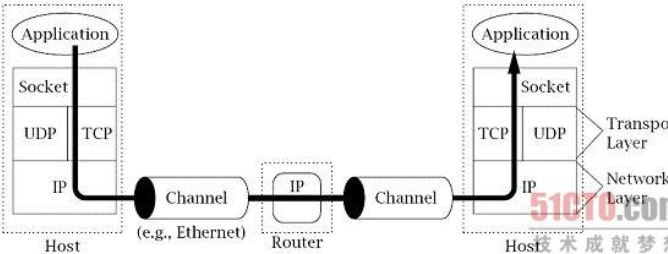
\includegraphics[scale=.6]{img/01.01.png}
			\caption{一个TCP/IP网络}
			\label{fig:tcpip.net.trans}
		\end{figure}

		Application:应用程序; Socket:套接字; Host:主机;Channel:通信信道; Ethernet:以太网; Router:路由器;Network Layer:网络层; Transport Layer:传输层。

		在 TCP/IP 协议族中,底层由基础的通信信道构成,如以太网或调制解调器拨号连接。这些信道由网络层(network layer)使用,而网络层则完成将分组报文传输到它们的目的地址的工作(也就是路由器的功能)。TCP/IP 协议族中属于网络层的唯一协议是 IP 协议,它使两个主机间的一系列通信信道和路由器看起来像是一条单一的主机到主机的信道。

		IP 协议提供了一种数据报服务:每组分组报文都由网络独立处理和分发,就像信件或包裹通过邮政系统发送一样。为了实现这个功能,每个 IP 报文必须包含一个保存其目的地址(address)的字段,就像你所投递的每份包裹都写明了收件人地址。(我们随即会对地址进行更详细的说明。)尽管绝大部分递送公司会保证将包裹送达,但 IP 协议只是一个"尽力而为"(best-effort)的协议:它试图分发每一个分组报文,但在网络传输过程中,偶尔也会发生丢失报文,使报文顺序被打乱,或重复发送报文的情况。

		IP 协议层之上称为传输层(transport layer)。它提供了两种可选择的协议:TCP 协议和UDP 协议。这两种协议都建立在 IP 层所提供的服务基础上,但根据应用程序协议(application protocols)的不同需求,它们使用了不同的方法来实现不同方式的传输。TCP 协议和 UDP协议有一个共同的功能,即寻址。回顾一下,IP 协议只是将分组报文分发到了不同的主机,很明显,还需要更细粒度的寻址将报文发送到主机中指定的应用程序,因为同一主机上可能有多个应用程序在使用网络。TCP 协议和 UDP 协议使用的地址叫做端口号(port numbers),都是用来区分同一主机中的不同应用程序。TCP 协议和 UDP 协议也称为端到端传输协议 (end-to-end transport protocols),因为它们将数据从一个应用程序传输到另一个应用程序,而 IP 协议只是将数据从一个主机传输到另一主机。

		TCP 协议能够检测和恢复 IP 层提供的主机到主机的信道中可能发生的报文丢失、重复及其他错误。TCP 协议提供了一个可信赖的字节流(reliable byte-stream)信道,这样应用程序就不需要再处理上述的问题。TCP 协议是一种面向连接(connection-oriented)的协议:在使用它进行通信之前,两个应用程序之间首先要建立一个 TCP 连接,这涉及到相互通信的两台电脑的 TCP 部件间完成的握手消息(handshake messages)的交换。使用 TCP 协议在很多方面都与文件的输入输出(I/O, Input/Output)相似。实际上,由一个程序写入的文件再由另一个程序读取就是一个 TCP 连接的适当模型。另一方面,UDP 协议并不尝试对 IP 层产生的错误进行修复,它仅仅简单地扩展了 IP 协议"尽力而为"的数据报服务,使它能够在应用程序之间工作,而不是在主机之间工作。因此,使用了 UDP 协议的应用程序必须为处理报文丢失、顺序混乱等问题做好准备。


	\section{关于地址}

		寄信的时候,要在表格中填上邮政服务能够理解的收信人的地址。在给别人打电话之前,必须给电话系统提供你所联系的人的电话号码。同样,一个程序要与另一个程序通信,就要给网络提供足够的信息,使其能够找到另一个程序。在 TCP/IP 协议中,有两部分信息用来定位一个指定的程序:互联网地址(Internet address)和端口号(port number)。其中互联网地址由 IP 协议使用,而附加的端口地址信息由传输协议(TCP 或 IP 协议)对其进行解析。

		互联网地址由二进制的数字组成,有两种型式,分别对应了两个版本的标准互联网协议。现在最常用的版本是版本 4, IPv4,即另一个版本是刚开始开发的版本 6, IPv6。即 IPv4 的地址长 32 位,只能区分大约 40 亿个独立地址,对于如今的互联网来说,这是不够大的。(也许看起来很多,但由于地址的分配方式的原因,有很多都被浪费了)出于这个原因引入了 IPv6,它的地址有 128 位长。

		为了便于人们使用互联网地址(相对于程序内部的表示),两个版本的 IP 协议有不同的表示方法。IPv4 地址被表示为一组 4 个十进制数,每两个数字之间由圆点隔开(如:10.1.2.3),这种表示方法叫做点分形式(dotted-quad)。点分形式字符串中的 4 个数字代表了互联网地址的 4 个字节,也就是说,每个数字的范围是 0 到 255。

		另一方面,IPv6 地址的 16 个字节由几组 16 进制的数字表示,这些 16 进制数之间由分号隔开(如:2000:fdb8:0000:0000:0001:00ab:853c:39a1)。每组数字分别代表了地址中的两个字节,并且每组开头的 0 可以省略,因此前面的例子中,第 5 组和第 6 组数字可以缩写为:1:ab:。甚至,只包含 0 的连续组可以全部省略(但在一个地址中只能这样做一次)。因此,前面的例子的完整地址可以表示为 2000:fdb8::1:00ab:853c:39a1。

		从技术角度来讲,每个互联网地址代表了一台主机与底层的通信信道的连接,换句话说,也就是一个网络接口(network interface)。主机可以有多个接口,这并不少见,例如一台主机同时连接了有线以太网(Ethernet)和无线网(WiFi)。由于每个这样的连接都属于唯一的一台主机,所以只要它连接到网络,一个互联网地址就能定位这条主机。但是反过来,一台主机并不对应一个互联网地址。因为每台主机可以有多个接口,每个接口又可以有多个地址。(实际上一个接口可以同时拥有 IPv4 地址和 IPv6 地址)。

		TCP 或 UDP 协议中的端口号总与一个互联网地址相关联。回到前面我们作类比的例子,一个端口号就相当于指定街道上一栋大楼的某个房间号。邮政服务通过街道地址把信分发到一个邮箱,再由清空邮箱的人把这封信递送到这栋楼的正确房间中。或者考虑一个公司的内部电话系统:要与这个公司中的某个人通话,首先要拨打该公司的总机电话号码连接到其内部电话系统,然后再拨打你要找的那个人的分机号码。在上面的例子中,互联网地址就相对于街道地址或公司的总机电话号码,端口号就相当于房间号或分机号码。端口号是一组 16位的无符号二进制数,每个端口号的范围是 1 到 65535。(0 被保留)。

		每个版本的 IP 协议都定义了一些特殊用途的地址。其中值得注意的一个是回环地址(loopback address),该地址总是被分配个一个特殊的回环接口(loopback interface)。回环接口是一种虚拟设备,它的功能只是简单地将发送给它的报文直接回发给发送者。回环接口在测试中非常有用,因为发送给这个地址的报文能够立即返回到目标地址。而且每台主机上都有回环接口,即使当这台计算机没有其他接口(也就是说没有连接到网络),回环接口也能使用。IPv4 的回环地址是 127.0.0.1[ ],IPv6 的回环地址是 0:0:0:0:0:0:0:1。

		IPv4 地址中的另一种特殊用途的保留地址包括那些"私有用途"的地址。它们包括 IPv4 中所有以 10 或 192.168 开头的地址,以及第一个数是 172,第二个数在 16 到 31 的地址。(在IPv6 中没有相应的这类地址)这类地址最初是为了在私有网络中使用而设计的,不属于公共互联网的一部分。现在这类地址通常被用在家庭或小型办公室中,这些地方通过 NAT(Network Address Translation,网络地址转换)设备连接到互联网。NAT 设备的功能就像一个路由器,转发分组报文时将转换(重写)报文中的地址和端口。更准确地说,它将一个接口中报文的私有地址端口对(private address, port pairs)映射成另一个接口中的公有地址端口对(public address, port pairs)。这就使一小组主机(如家庭网络)能够有效地共享同一个 IP 地址。重要的是这些内部地址不能从公共互联网访问。如果你在拥有私有类型地址的计算机上试验本书的例子,并试图与另一台没有这类地址的主机进行通信,通常只有这台拥有私有类型地址的主机发起的通信才能成功。

		相关的类型的地址包括本地链接(link-local),或称为"自动配置"地址。IPv4 中,这类地址由 169.254 开头,在 IPv6 中,前 16 位由 FE8 开头的地址是本地链接地址。这类地址只能用来在连接到同一网络的主机之间进行通信,路由器不会转发这类地址的信息。最后,另一类地址由多播(multicast)地址组成。普通的 IP 地址(有时也称为"单播"地址)只与唯一一个目的地址相关联,而多播地址可能与任意数量的目的地址关联。我们将在第 4 章中简要地对多播技术作进一步介绍。IPv4 中的多播地址在点分格式中,第一个数字在 224 到 239 之间。IPv6 中,多播地址由 FF 开始。 

	\section{关于名字}

		也许你更习惯于通过名字来指代一个主机,例如:host.example.com。然而,互联网协议只能处理二进制的网络地址,而不是主机名。首先应该明确的是,使用主机名而不使用地址是出于方便性的考虑,这与TCP/IP提供的基本服务是相互独立的。你也可以不使用名字来编写和使用TCP/IP应用程序。当使用名字来定位一个通信终端时,系统将做一些额外的工作把名字解析成地址。有两个原因证明这额外的步骤是值得的:

		第一,相对于点分形式(或IPv6中的十六进制数字串),人们更容易记住名字;

		第二,名字提供了一个间接层,使IP地址的变化对用户不可见。在本书第一版的写作期间,网络服务器www.mkp.com的地址就改变过。

		由于我们通常都使用网络服务器的名字,而且地址的改变很快就被反应到映射主机名和网络地址的服务上(我们马上会对其进行更多的介绍),如www.mkp.com从之前的地址208.164.121.48 对应到了现在的地址,这种变化对通过名字访问该网络服务器的程序是透明的。

		名字解析服务可以从各种各样的信息源获取信息。两个主要的信息源是域名系统(DNS,Domain Name System)和本地配置数据库。DNS[ ]是一种分布式数据库,它将像www.mkp.com这样的域名映射到真实的互联网地址和其他信息上。DNS协议允许连接到互联网的主机通过TCP或UDP协议从DNS数据库中获取信息。本地配置数据库通常是一种与具体操作系统相关的机制,用来实现本地名称与互联网地址的映射。

	\section{客户端和服务器}
		在前面的邮政和电话系统例子中,每次通信都是由发信方或打电话者发起,而另一方则通过发回反馈信或接听电话来对通信的发起者作出响应。互联网通信也与这个过程类似。客户端(client)和服务器(server)这两个术语代表了两种角色:客户端是通信的发起者,而服务器程序则被动等待客户端发起通信,并对其作出响应。客户端与服务器组成了应用程序(application)。客户端和服务器这两个术语对典型的情况作出了描述,服务器具有一定的特殊能力,如提供数据库服务,并使任何客户端能够与之通信。

		一个程序是作为客户端还是服务器,决定了它在与其对等端(peer)建立通信时使用的套接字 API 的形式(客户端的对等端是服务器,反之亦然)。更进一步来说,客户端与服务器端的区别非常重要,因为客户端首先需要知道服务器的地址和端口号,反之则不需要。如果有必要,服务器可以使用套接字 API,从收到的第一个客户端通信消息中获取其地址信息。这与打电话非常相似:被呼叫者不需要知道拨电话者的电话号码。就像打电话一样,只要通信连接建立成功,服务器和客户端之间就没有区别了。

		客户端如何才能找到服务器的地址和端口号呢?通常情况,客户端知道服务器的名字,例如使用URL(Universal Resource Locator,统一资源定位符)如http://www.mkp.com,再通过名字解析服务获取其相应的互联网地址。

		获取服务器的端口号则是另一种情况。从原理上来讲,服务器可以使用任何端口号,但客户端必须能够获知这些端口号。在互联网上,一些常用的端口号被约定赋给了某些应用程序。例如,端口号 21 被FTP(File Transfer Protocol,文件传输协议)使用。当你运行FTP客户端应用程序时,它将默认通过这个端口号连接服务器。互联网的端口号授权机构维护了一个包含所有已约定使用的端口号列表(见http://www.iana.org/assignments/port-numbers)。

	\section{什么是套接字}

		Socket(套接字)是一种抽象层,应用程序通过它来发送和接收数据,就像应用程序打开一个文件句柄,将数据读写到稳定的存储器上一样。一个 socket 允许应用程序添加到网络中,并与处于同一个网络中的其他应用程序进行通信。一台计算机上的应用程序向 socket写入的信息能够被另一台计算机上的另一个应用程序读取,反之亦然。

		不同类型的 socket 与不同类型的底层协议族以及同一协议族中的不同协议栈相关联,本书只涵盖了 TCP/IP 协议族的内容。现在 TCP/IP 协议族中的主要 socket 类型为流套接字(sockets sockets)和数据报套接字(datagram sockets)。流套接字将 TCP 作为其端对端协议(底层使用 IP 协议),提供了一个可信赖的字节流服务。一个 TCP/IP 流套接字代表了 TCP 连接的一端。数据报套接字使用 UDP 协议(底层同样使用 IP 协议),提供了一个"尽力而为"(best-effort)的数据报服务,应用程序可以通过它发送最长 65500 字节的个人信息。当然,其他协议族也支持流套接字和数据报套接字,但本书只对 TCP 流套接字和 UDP 数据报套接字进行讨论。一个 TCP/IP 套接字由一个互联网地址,一个端对端协议(TCP 或 UDP 协议)以及一个端口号唯一确定。随着进一步学习,你将了解到把一个套接字绑定到一个互联网地址上的多种方法。

		图 1.2 描述了一个主机中,应用程序、套接字抽象层、协议、端口号之间的逻辑关系。
		\begin{figure}[htbp]%位置选项
			\centering
			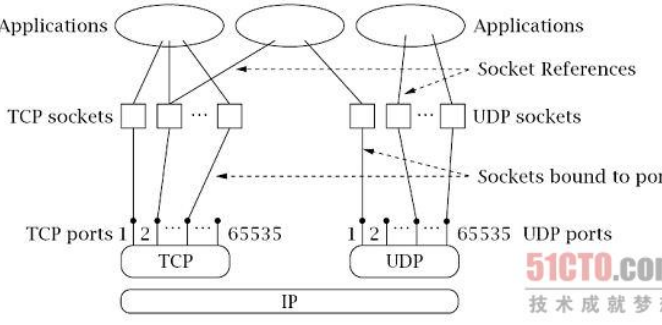
\includegraphics[scale=.6]{img/01.02.png}
			\caption{套接字、协议、端口}
			\label{fig:socket.trans}
		\end{figure}

		Applications:应用程序;TCP sockets:TCP 套接字;TCP ports:TCP 端口;Socket References:套接字引用;UDP sockets:UDP 套接字;Sockets bound to ports:套接字绑定到 端口;UDP ports:UDP 端口。

		值得注意的是一个套接字抽象层可以被多个应用程序引用。每个使用了特定套接字的程序都可以通过那个套接字进行通信。前面已提到,每个端口都标识了一台主机上的一个应用程序。实际上,一个端口确定了一台主机上的一个套接字。从图 1.2 中我们可以看到,主机中的多个程序可以同时访问同一个套接字。在实际应用中,访问相同套接字的不同程序通常都属于同一个应用(例如,Web 服务程序的多个拷贝),但从理论上讲,它们是可以属于不同应用的。




	\part{Java API}

		
\chapter{基本套接字}

	\section{套接字地址}

		\subsection{例子}

		\lstinputlisting[]{src/ch02/InetAddressExample.java}

		运行与输出结果:

\begin{lstlisting}[language=Bash]
% java InetAddressExample \
	www.baidu.com www.jadehahaha.com \
	129.35.69.7

Interface eth0:
	Address (v6): fe80:0:0:0:225:b3ff:fe69:1659%2
	Address (v4): 172.16.7.1
Interface lo:
	Address (v6): 0:0:0:0:0:0:0:1%1
	Address (v4): 127.0.0.1
www.baidu.com: 
	www.baidu.com/220.181.111.147
www.jadehahaha.com: 
	Unable to find address for : www.jadehahaha.com
129.35.69.7: 
	129.35.69.7/129.35.69.7
\end{lstlisting}

		\subsection{InetAddress类API简介}

			InetAddress类中创建与访问实例方法:
\begin{lstlisting}
static InetAddress [] getAllByName(String host);
static InetAddress getByName(String host);
static InetAddress getLocalHost();
/**
 * return byte array as ip address
 * size if 4 byte in ipv4
 * or size is 16 in ipv6
 */
byte[] getAddress();
\end{lstlisting}

			InetAddress类中字符串显示方法:
\begin{lstlisting}
/**
 * return value format like:
 *   hostname.example.com/192.0.2.127
 *   or
 *   never.example.net/2000::620:1a30:95b2
 */
String toString();
String getHostAddress();
/**
 * return host name
 */
String getHostName();
/**
 * return host name ()
 */
String getCanonicalHostName();
\end{lstlisting}

			InetAddress类中检查属性的方法:
\begin{lstlisting}
boolean isAnyLocalAddress();
boolean isLinkLocalAddress();
boolean isLoopBackAddress();
// 是否为多播地址
boolean isMulticastAddress();
// 测试多播地址范围:global
boolean isMCGlobal();
// 测试多播地址范围:link local
boolean isMCLinkLocal();
// 测试多播地址范围:node local
boolean isMCNodeLocal();
// 测试多播地址范围:org local
boolean isMCOrgLocal();
// 测试多播地址范围:site local
boolean isMCSiteLocal();
boolean isReachable(int timeout);
boolean isReachable(NetworkInterface netif, int ttl, int timeout)
\end{lstlisting}


	\section{TCP套接字}


	\part{其他扩展}

% \chapter{基本使用}
% 
% 	\section{常用的格式}
% 
% 		\subsection{基本的段落}
% 			空行可以自然分隔段落:
% 
% 			可以设定字体为\textit{斜体};给文字加上\underline{下划线}。可以设定字体为\textit{斜体};给文字加上\underline{下划线}。可以设定字体为\textit{斜体};给文字加上\underline{下划线}。可以设定字体为\textit{斜体};给文字加上\underline{下划线}。
% 
% 			可以设定字体为\textit{斜体};给文字加上\underline{下划线}。可以设定字体为\textit{斜体};给文字加上\underline{下划线}。可以设定字体为\textit{斜体};给文字加上\underline{下划线}。可以设定字体为\textit{斜体};给文字加上\underline{下划线}。
% 
% 			可以设定字体为\textit{斜体};给文字加上\underline{下划线}。可以设定字体为\textit{斜体};给文字加上\underline{下划线}。可以设定字体为\textit{斜体};给文字加上\underline{下划线}。可以设定字体为\textit{斜体};给文字加上\underline{下划线}。
% 
% 		\subsection{边注与脚注}
% 			按照国际惯例,这里是鬼扯的部分。\footnote{我才不承认这是为了骗稿费呢~}
% 
% 			同样也给内容加上连注。但边注是没有编号的,因为就在旁边。\marginpar{这里是边注的内容。}
% 
% 		\subsection{原文照排}
% 			在正文中放入源文照排:在Linux下通过\verb|ls -al|查看当前目录下所有文件。
% 
% 			多行的原文照排要用到verbatim环境:
% 			\begin{verbatim}
% 				/* 输出10行"Hello, world!"的面试题 */
% 				/* 某位童鞋的答案是这样写的        */
% 				printf("Hello, world!");
% 				printf("Hello, world!");
% 				printf("Hello, world!");
% 				printf("Hello, world!");
% 				printf("Hello, world!");
% 				printf("Hello, world!");
% 				printf("Hello, world!");
% 				printf("Hello, world!");
% 				printf("Hello, world!");
% 				printf("Hello, world!");
% 			\end{verbatim}
% 
% 			原文照排时强调空格到verbatim*环境:
% 			\begin{verbatim*}
% 				printf("Hello, world!");
% 			\end{verbatim*}
% 
% 		\subsection{程序代码}
% 
% 			使用listings宏包的效果:
% 
% \begin{lstlisting}[language=C]
% #include <stdio.h>
% 
% int main(int argc, char ** argv)
% {
% 	printf("Hello world!\n");
% 	/** 看起来直接用listings和xelatex配合显示中文没有问题 **/
% 	printf("显示中文!\n");
% 	return 0;
% }
% \end{lstlisting}
% 
% 			可以只引用整个代码中的一部分:
% 
% \begin{lstlisting}[language=C,firstline=3,lastline=9]
% #include <stdio.h>
% 
% int main(int argc, char ** argv)
% {
% 	printf("Hello world!\n");
% 	/** 看起来直接用listings和xelatex配合显示中文没有问题s1l1O0O0 **/
% 	printf("显示中文!\n");
% 	return 0;
% }
% \end{lstlisting}
% 
% 			使用\verb|\lstinputlisting|引用外部文件:
% 
% 			\lstinputlisting[language=HTML,firstline=2,lastline=8]{src/aa.html}
% 
% 	\section{图片与表格}
% 
% 		\subsection{使用图片}
% 
% 			试试使用浮动环境插入图片,但是这样图片就不知道浮动到什么地方去了:
% 
% 			\begin{figure}[htbp]                        % 
% 				\centering                              % 图片居中	
% 				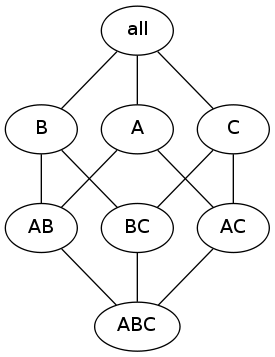
\includegraphics[scale=0.5]{dm0201.png} % scale指定缩放
% 				\caption{第一张浮动的图片}            % 图片的标题,会自动编号
% 				\label{dm0201}                % 图片的标记,一定要加在caption后面。不然指向的是前一个插图
% 			\end{figure}
% 
% 			试试使用浮动环境插入图片,但是这样图片就不知道浮动到什么地方去了:
% 
% 			\begin{figure}[htbp]                        % 
% 				\centering                              % 图片居中	
% 				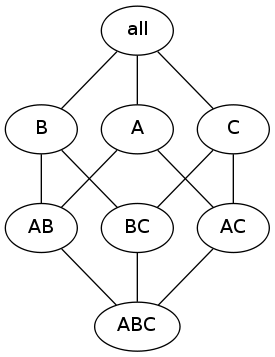
\includegraphics[scale=0.5]{dm0201.png} % scale指定缩放
% 				\caption{第二张浮动的图片}            % 图片的标题,会自动编号
% 				\label{dm0202}                % 图片的标记,一定要加在caption后面。不然指向的是前一个插图
% 			\end{figure}
% 
% 			试试使用浮动环境插入图片,但是这样图片就不知道浮动到什么地方去了:
% 
% 			\begin{figure}[htbp]                        % 
% 				\centering                              % 图片居中	
% 				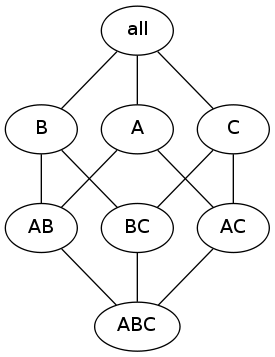
\includegraphics[scale=0.5]{dm0201.png} % scale指定缩放
% 				\caption{第三张浮动的图片}            % 图片的标题,会自动编号
% 				\label{dm0203}                % 图片的标记,一定要加在caption后面。不然指向的是前一个插图
% 			\end{figure}
% 
% 		\subsection{使用表格}
% 
% 			组表格也加上浮动环境:
% 
% 			\begin{table}[htbp]
% 				\caption{浮动环境中的三线表}
% 				\label{tab:threesome}
% 				\centering
% 				\begin{tabular}{lll}
% 					\hline
% 					操作系统 & 发行版 & 编辑器 \\
% 					\hline
% 					Windows & MikTeX & TeXnicCenter \\
% 					Unix/Linux & TeX Live & Emacs \\
% 					Mac OS & MacTeX & TeXShop \\
% 					\hline
% 				\end{tabular}
% 			\end{table}
% 

\end{document}
